\documentclass[11pt]{article}
\usepackage[a4paper,margin=25mm]{geometry}
\usepackage{amsmath,amssymb,graphicx,booktabs,tabularx,array}
\usepackage[round,authoryear]{natbib}
\usepackage[font=small,labelfont=bf]{caption}
\usepackage[colorlinks=true,allcolors=blue]{hyperref}
\usepackage{microtype,flafter,placeins}
\graphicspath{{figures/}}
\setlength{\parindent}{1em}
\setlength{\parskip}{2pt}
\setlength{\emergencystretch}{2em}
\clubpenalty=10000
\widowpenalty=10000
\renewcommand{\topfraction}{0.9}
\renewcommand{\bottomfraction}{0.8}
\renewcommand{\textfraction}{0.08}
\renewcommand{\floatpagefraction}{0.75}
\newcommand{\E}{\widehat{\mathcal E}}
\newcommand{\R}{\mathbb R}
\title{Artist-Name Responses beyond a Shared Painting Effect\\in Text-to-Image Generation}
\author{Anonymous authors}
\date{}
\begin{document}
\maketitle

\begin{abstract}
A detectable response to a painter's name need not reproduce differences
between painters. We test this distinction in 31 digital color, spatial and
texture features using 649 reproductions of Monet, Sisley, Pissarro and
C\'ezanne. Six generators receive 14 fixed outdoor briefs under artist-free,
generic-painting and four named-painter conditions, with two outputs per cell.
After removing the common additive response, all six configurations have
positive reference-aligned slopes, but alignment is uneven across artist pairs.
GPT Image 2 nearly matches aggregate aligned amplitude ($\beta=.999$) while
retaining substantial error ($D=1.226$). FLUX.2 Max has the lowest primary error
estimate and adjusted advantages over the two GPT Image 2.5 configurations;
no model is established to beat the no-artist-contrast benchmark. Scalar
calibration on other scenes instead gives GPT Image 2 the lowest held-scene
point estimate. Source-region correction retains FLUX's lowest point estimate
but removes adjusted separation from Sunburst. The contribution is a controlled separation of name response,
calibration and agreement with a specified reference collection, rather than
a validated ranking of artistic fidelity.
\end{abstract}

\section{Introduction}
A painter's name can change an image in several ways. It can introduce a common
painting appearance, exaggerate familiar color or texture cues, or alter the
features that distinguish one painter from another. These effects are easy to
conflate. Moving closer to Monet's collection, for example, does not show that
a generator reproduces the differences between Monet and Sisley: a generic
painting instruction could improve proximity to both.

We ask whether painter names induce differences aligned with those among
\emph{documented digital reproductions}, beyond a response shared across names.
Our target is the labeled, centered mean configuration of four painters in
31 color, spatial and texture coordinates. This is an explicit collection-relative
target, not a perceptually validated definition of style. Historical subject
mixtures and reproduction processes can contribute to its artist differences.
Holding the generated scene text fixed controls the prompt intervention; it
does not make those historical subjects identical.

The distinction matters for evaluation. A generator can produce easily
separable named conditions whose labels map to the wrong reference painters.
It can also recover the reference-aligned amplitude while introducing large
additional contrasts. Conversely, a restrained response may have lower squared
error than a stronger response, without distinguishing artists more accurately
in every respect. A single proximity score or recognition accuracy cannot
separate these possibilities.

We cross six model configurations with identical scene descriptions and
artist-free, generic oil-painting and four named-painter clauses. Centering
removes their common additive shift; a projection measures reference-aligned
amplitude, and an independent-repeat cross-product estimates scene-wise
squared disagreement without additive sampling-noise bias. The results reveal
uneven artist-pair alignment and model orderings that change with response
calibration and scene dependence. Separate post-result diagnostics examine
these distinctions and reference quality. The contribution is this controlled
empirical audit using established estimators.

\section{Related work}
\citet{somepalli2024style} develop learned style descriptors and study similarity
across diffusion models. \citet{su2025prompted} evaluate prompted-artist
recognition using content-controlled name substitutions and compare named and
artist-free images with real-artist prototypes in CLIP space. Our question
concerns the labeled differences among reference painters after removing a
shared response; neither name substitution nor cross-model comparison is new.

\citet{deliege2025} assess stylistic imitation and stereotyping with experts.
AI-Pastiche studies authenticity judgments and prompt adherence
\citep{asperti2025pastiche}, while AI-WikiArt uses painting-derived captions and
vision-language models for attribution \citep{fu2025aiwikiart}. These tasks
distinguish convincing imitation, recognizable authorship and distributional
agreement. Here, the evaluation target is explicitly the latter in measured
color, spatial and texture coordinates.

Quantitative art research studies color, composition and image statistics
\citep{kim2014,sigaki2018,lee2020}. \citet{kim2026} combine formal and contextual
representations for art-historical analysis and contextual image-to-image
experiments. Our text-only name intervention supplies no original composition;
its common scenes control requested generated content, not historical subjects.

Generative evaluation separates fidelity and diversity \citep{naeem2020},
and conditional metrics separate within-condition variation from relationships
among means \citep{benny2021conditional}. Independent-partition inner products
provide noise-corrected squared differences \citep{diedrichsen2017representational};
energy statistics supply a complementary distributional measure \citep{szekely2013}.
Processing sensitivity \citep{parmar2022} and limits of learned-embedding
separation \citep{asperti2026} motivate the source-quality checks and the
restriction to a specified digital reference target.

\section{Design and measurements}\label{sec:design}
\subsection{Painters and reference images}
The primary panel comprises 649 distinct painting reproductions: 297 Monet,
106 Sisley, 141 Pissarro and 105 C\'ezanne. Artist means receive equal weight,
so the larger Monet collection does not dominate the between-artist target.
A separate development panel of 221 works supplies feature scaling; no primary
reference or generated image is used to fit that transformation. Both panels
were assembled before the present experiment and had been used in earlier
analyses. They are explicit, finite comparison panels rather than newly withheld
samples of each painter's complete oeuvre.

Reference files carry Wikimedia Commons source metadata and Wikidata work
identities \citep{commonsglam,vrandecic2014wikidata}. These support traceable
selection and rights records, but do not standardize photography, color
calibration or conservation state. The Web Gallery of Art in \citet{kim2014},
ART500K in \citet{kim2026} and WikiArt in \citet{fu2025aiwikiart} are different
corpora, not validations of this collection. We therefore distinguish digital
reproductions from the physical paintings.

\subsection{A common-scene, six-model experiment}
We compare GPT Image 1, GPT Image 2, GPT Image 2.5 Flare, GPT Image 2.5 Sunburst,
Nano Banana 2 and FLUX.2 Max. Fourteen authored outdoor scenes span water,
built, land and mixed compositions. Each scene is crossed with six clauses:
no painting instruction; ``Render as an oil painting''; and ``Render as an oil
painting in the style of [painter]'' for each of the four painters. The scene
text is otherwise identical. Each model--scene--clause cell receives two
separately requested outputs, giving 1,008 images collected on 10 September 2026.

All models receive text only and return 1,024-by-1,024-pixel images.
The four OpenAI models use medium quality; the other two use
their specified 1K configurations. These comparisons concern the recorded
configurations, not maximum attainable quality or equal expenditure per image.
The exact prompts, parameters and randomized request order were fixed before
collection. The 14 scenes are a fixed design,
not a random sample of all possible content.

\subsection{What the features measure}\label{sec:features}
Images undergo orientation correction and conversion to sRGB using valid
embedded profiles; compatible unprofiled files are treated as sRGB. The primary
pipeline preserves aspect ratio at a 512-pixel short side, using Lanczos resizing
without upsampling. No painting-region mask is applied: source margins or
calibration strips can enter the measurements. Each coordinate is centered and scaled by its
median and interquartile range in the development panel, with equal total
weight per painter. Thus a unit is a development-panel IQR in that coordinate,
not a perceptual just-noticeable difference. The Euclidean metric weights
standardized coordinates equally, without further equalizing feature families.

Table~\ref{tab:features} explains the representation. Color features summarize
lightness and chroma, concentration of hue, and color changes across spatial
scales; CIEDE2000 supplies the color-difference calculation
\citep{sharma2005ciede}. Spatial features describe how luminance contrast is
organized across frequencies, directions and regions. Texture features summarize
multiscale detail and local intensity patterns using wavelets and local binary
patterns \citep{mallat1989wavelet,ojala2002lbp}. For example, similar mean chroma
can coexist with different hue diversity, and similar total contrast can coexist
with different edge orientation or fine-scale texture. These distinctions make
family-specific results interpretable, while correlated coordinates and
processing sensitivity prevent treating the Euclidean metric as a validated
measure of artistic style.

\begin{table}[tbp]
\centering\small
\begin{tabularx}{\linewidth}{@{}>{\raggedright\arraybackslash}p{.15\linewidth}>{\raggedright\arraybackslash}p{.35\linewidth}>{\raggedright\arraybackslash}X@{}}
\toprule
Family & Measurements & Interpretation\\
\midrule
Color (11) & Lightness and chroma median/IQR; chromatic fraction; hue
concentration and entropy; color differences at three lags and their slope &
Brightness, color strength and diversity, and how rapidly colors change over space.\\[4pt]
Spatial (8) & Spectral slope, residual and anisotropy; orientation entropy;
horizontal--vertical balance; gradient median/IQR; quadrant divergence &
Coarse versus fine organization, dominant directions, edge strength and regional
variation in orientation.\\[4pt]
Texture (12) & Four wavelet energies, slope and curvature; three local-binary-pattern
entropies; three local coefficients of variation &
Detail across scales, diversity of local patterns and local luminance contrast.\\
\bottomrule
\end{tabularx}
\caption{The 31 fixed digital features. Counts refer to scalar coordinates.
Texture measurements do not measure physical paint relief or authenticate brushwork.
Exact scales and definitions appear in Appendix~\ref{app:features}.}
\label{tab:features}
\end{table}

\section{Measuring reference-relative artist contrasts}\label{sec:method}
\subsection{Reference-aligned variation}
Let $\mu_a\in\R^{31}$ be the standardized reference mean for painter $a$ and
let $\bar\mu=\frac14\sum_a\mu_a$. Define the reference painter contrasts
$r_a=\mu_a-\bar\mu$ and their total squared magnitude $H=\sum_a\|r_a\|^2$.
For generated vector $z_{msak}$ from model $m$, scene $s$, painter $a$ and
repeat $k\in\{1,2\}$, remove the common additive named response:
\begin{equation}
 d_{msak}=z_{msak}-\frac14\sum_b z_{msbk}.
 \label{eq:center}
\end{equation}
Any shift shared by all four named outputs of that model, scene and repeat
cancels exactly. This removes additive baselines in these coordinates. It does not remove
a shared transformation: if all conditions undergo $z\mapsto Az+b$,
centering removes $b$ but leaves $Ad$.

The reference-aligned slope is
\begin{equation}
 \widehat\beta_{msk}=\frac{\sum_a\langle d_{msak},r_a\rangle}{H},\qquad
 \widehat\beta_m=\frac1S\sum_s\frac{\widehat\beta_{ms1}+\widehat\beta_{ms2}}2.
 \label{eq:beta}
\end{equation}
It is the least-squares coefficient of generated painter contrasts on reference
contrasts. A value of zero indicates no response along the reference direction;
one matches its amplitude. Values above one indicate exaggeration along that
direction, not necessarily better recovery. A nonzero slope does not establish agreement for every artist pair. It is
a projection onto one vectorized reference configuration, not a test that
all reference contrast dimensions are recovered.

\subsection{Repeat-corrected disagreement with a pooled target}
Two independently requested repeats permit the cross-product estimator
\begin{equation}
 \widehat D_{ms}=\frac1H\sum_a
 \langle d_{msa1}-r_a,\ d_{msa2}-r_a\rangle,\qquad
 \widehat D_m=\frac1S\sum_s\widehat D_{ms}.
 \label{eq:distortion}
\end{equation}
Under stable conditional means and independent, mean-zero repeat errors, its
expectation is the squared error of the scene-conditional mean painter
contrasts, normalized by $H$. The error contributed by output sampling does not
inflate this expectation. Exact agreement with these reference contrasts in every scene gives expected
$D=0$; identical conditional means for all four artist labels give expected
$D=1$. This latter benchmark is a theoretical no-contrast predictor, not an
observed generic-arm estimate. Finite estimates may be
negative. We do not truncate them or interpret a negative estimate as
better-than-perfect recovery.

The estimator has an exact decomposition. Write
$e_{msak}=d_{msak}-\widehat\beta_{msk}r_a$. Then
\begin{equation}
 \widehat D_{ms}=
 (\widehat\beta_{ms1}-1)(\widehat\beta_{ms2}-1)
 +\frac1H\sum_a\langle e_{msa1},e_{msa2}\rangle.
 \label{eq:decomposition}
\end{equation}
The first term measures reference-aligned amplitude error. The residual is
orthogonal to the single stacked reference configuration; it is not necessarily
outside the feature-space span of the reference means, much less outside all
authentic artistic variation. Both terms can be negative in finite samples.

A simple example clarifies the target. Conditional contrasts $0$, $r$ and $2r$
give expected errors 1, 0 and 1, respectively. Permuting distinct reference
labels preserves all unlabeled pairwise distances but gives nonzero error.
Thus $D$ measures labeled coordinate agreement, including response strength.
It is not just a measure of separation or distance-geometry preservation.

Let $\theta_s$ stack the four conditional mean contrasts and
$\bar\theta=S^{-1}\sum_s\theta_s$. The population target decomposes as
\begin{equation}
 D_{\rm scene}=\frac{\|\bar\theta-r\|^2}{H}
 +\frac1{SH}\sum_s\|\theta_s-\bar\theta\|^2
 =D_{\rm aggregate}+V_{\rm scene}.
 \label{eq:scene-decomposition}
\end{equation}
The second term penalizes changes in artist contrasts across scenes. Such
changes need not be artistic mistakes: a generator with $\theta_s=r+u_s$
and $\sum_su_s=0$ matches the aggregate target but incurs positive scene-wise
error. We therefore interpret the primary endpoint as \emph{scene-wise agreement
with pooled reference contrasts}. It cannot establish content-conditional
artist fidelity without a corresponding historical target.

\subsection{Comparing models}
We fit the scene fixed-effects regression
\begin{equation}
 \widehat D_{ms}=\alpha_s+\gamma_m+\varepsilon_{ms},
 \qquad\gamma_{\text{GPT Image 2}}=0.
 \label{eq:regression}
\end{equation}
All models face the same scenes and equally weighted reference painter target.
With a complete balanced panel, model coefficient differences equal the mean
paired scene differences. Inference uses those scene differences rather than
treating features, painters or individual images as independent replicates.

The fixed inferential family contains six reference-aligned slopes and 15
pairwise model error contrasts. We report paired-scene Student intervals with
$n-1$ degrees of freedom and Bonferroni adjustment across these 21 comparisons.
Nominal 95\% intervals for absolute $D_m$ are descriptive. These are approximate
model-based summaries using dispersion across the fixed briefs. That dispersion
mixes generation noise with genuine between-brief variation in conditional
contrasts; it does not isolate fresh-request uncertainty for exactly these
briefs or establish coverage for new scenes. Bonferroni adjustment requires
adequately calibrated individual intervals. Two outputs permit noise correction
but do not precisely characterize its sampling distribution. All 14 scenes
are complete for all models.

Prespecified sensitivity analyses remove each scene in turn, resample scenes
for model contrasts, and resample reference works within painter while holding
generated vectors fixed. The last analysis assesses dependence on this reference
panel; it is not a second independent uncertainty estimate. We also repeat the
analysis in each feature family, without texture, and using central square
measurement windows for both generated and reference images. The square view
controls measurement-window aspect ratio while discarding peripheral content.
These analyses are descriptive and do not select a preferred representation.

A separately declared sensitivity addresses unequal subject mixtures in the
references. Before inspecting the new feature outcomes, we specified equal
weight for four previously recorded, metadata-derived content classes within each painter, then
recomputed the reference contrasts and all model estimates. For example, water
scenes are much more frequent in the Monet panel than in the Pissarro panel.
Equal class weighting changes the pooled mixture; it does not supply a
content-conditional target, match individual compositions or identify pure style. Reference resampling within
artist/class strata assesses the stability of this alternative target.

\subsection{Generic controls and full distributions}
The mean change from the free arm to the four named arms separates into a common
component and centered painter contrasts. We compare the direction and magnitude
of the common component with the free-to-generic change. Cross-repeat squared magnitudes and alignment
ratios assess how much of the shared direction a generic painting clause reproduces;
ordinary cosines are retained as descriptive comparisons. A large common fraction alone cannot show that
naming fails: these four reference painters also share visual properties.
Equations~\ref{eq:beta}--\ref{eq:distortion} separately assess reference contrasts.

For painter $a$, energy discrepancy compares its generated collection $Y_a$
with reference collection $X_a$:
\begin{equation}
 \E(X,Y)=\frac{2}{n_Xn_Y}\sum_{i,j}\|x_i-y_j\|
 -\frac1{n_X^2}\sum_{i,i'}\|x_i-x_{i'}\|
 -\frac1{n_Y^2}\sum_{j,j'}\|y_j-y_{j'}\|.
 \label{eq:energy}
\end{equation}
Unlike distance to a mean, this statistic incorporates within-collection
variation. Its finite-sample expectation depends on within-collection spread, so equal
generated sample sizes do not eliminate comparison bias. We retain this declared
statistic and add a correction respecting the scene-stratified design in
Appendix~\ref{app:diagnostics}. Generated/reference variance ratios compare
28 outputs from 14 fixed briefs with a historically broader collection. A ratio
below one is not, by itself, evidence of deficient diversity. We also
report within-scene repeat spread, $\frac{1}{2S}\sum_s
\|z_{msa1}-z_{msa2}\|^2$, the mean sample-variance trace of the two repeated
outputs. This separates repeat dispersion from total variation across briefs.

\subsection{Post-result diagnostic analyses}\label{sec:diagnostics}
The declared endpoints are retained. The following analyses were added in
response to review, after the primary results were known, and are descriptive.
We examine artist pairs, reference singular components, label permutations,
class-specific targets and disjoint real/reference controls. Subsequent checks
separate control-sampling noise, correct shared-control alignment, and audit
reference regions and labels. Weighting sensitivities and explicit noise
simulations assess numerical stability. Appendix~\ref{app:diagnostics} specifies
these retrospective analyses; full records accompany the code.

To separate contrast strength from direction, define
\begin{equation}
 \widehat Q_m=\frac1{SH}\sum_{s,a}\langle d_{msa1},d_{msa2}\rangle,
 \qquad \widehat D_m=1-2\widehat\beta_m+\widehat Q_m.
 \label{eq:magnitude}
\end{equation}
For positive $\widehat Q_m$, $\widehat\beta_m/\sqrt{\widehat Q_m}$ is a
noise-corrected alignment summary; finite estimates need not lie in $[-1,1]$.
Scaling every centered generated contrast by $c$ gives
$\widehat D_m(c)=1-2c\widehat\beta_m+c^2\widehat Q_m$.
We fit $c=\max(0,\widehat\beta/\widehat Q)$ on the other 13 scenes and evaluate
it on the held-out scene. The fitting criterion is available only when its
training $\widehat Q$ is positive, as it is in every observed fold. This
counterfactual concerns feature vectors, not an implemented image transformation.

\section{Results}\label{sec:results}
\subsection{A response in the right direction can still miss the target}
All 1,008 outputs yield valid measurements. With the full-frame
reference target, every model's aligned-response interval lies above zero
(Table~\ref{tab:specificity-models}). A purely common additive response is
therefore insufficient to explain the named conditions under the stated
inference model. Yet positive alignment does not ensure low error. GPT Image 2
nearly matches the reference-aligned strength, $\beta=.999\;[.893,1.104]$,
while its total error is $D=1.226$: it adds substantial differences beyond
that aligned component.

\begin{table}[tbp]
\centering\small\setlength{\tabcolsep}{4pt}
\begin{tabularx}{\linewidth}{@{}>{\raggedright\arraybackslash}p{.24\linewidth}>{\raggedright\arraybackslash}Xr>{\raggedright\arraybackslash}X@{}}
\toprule
Model & Aligned response $\beta$ & \shortstack{Uncalibrated\\error $D$} & $\Delta D$ versus FLUX\\
\midrule
GPT Image 1 & $0.938\;[0.709,1.168]$ & $1.572$ & $0.771\;[-0.037,1.580]$\\[3pt]
GPT Image 2 & $0.999\;[0.893,1.104]$ & $1.226$ & $0.425\;[-0.161,1.011]$\\[3pt]
GPT Image 2.5 Flare & $0.772\;[0.680,0.864]$ & $1.738$ & $0.937\;[0.256,1.618]$\\[3pt]
GPT Image 2.5 Sunburst & $0.824\;[0.680,0.968]$ & $1.641$ & $0.840\;[0.058,1.623]$\\[3pt]
Nano Banana 2 & $0.442\;[0.256,0.629]$ & $1.109$ & $0.309\;[-0.847,1.464]$\\[3pt]
FLUX.2 Max & $0.470\;[0.239,0.701]$ & $0.801$ & $0$ (baseline)\\[3pt]
\bottomrule\end{tabularx}
\caption{Agreement with the full-frame reference target. $\beta=1$ matches its aligned amplitude; larger is not necessarily better. Expected $D$ is 0 for exact agreement and 1 for no painter distinctions. Positive $\Delta D$ favors FLUX.2 Max. Table brackets give approximate 95\% simultaneous intervals from the prespecified family of six aligned responses and 15 scene-paired model contrasts. FLUX's lowest $D$ estimate has an unadjusted 95\% interval $[0.586,1.016]$, spanning the no-distinction value 1; this interval is descriptive.}
\label{tab:specificity-models}\end{table}


FLUX.2 Max has the lowest error estimate, $.801$, despite a smaller aligned
response, $.470$. Adjusted comparisons resolve higher error for Flare and Sunburst
than for FLUX; the other 13 intervals include zero (Appendix~\ref{app:results},
Table~\ref{tab:all-specificity-pairs}).
These use full-frame references;
the Sunburst result changes after source correction
(Section~\ref{sec:source-correction}). No model is established to beat the
no-contrast benchmark of one. Thus the study detects a
reference-aligned response more clearly than it establishes low total mismatch.

In Figure~\ref{fig:specificity-geometry}, C\'ezanne remains visibly separated,
while generated Monet and Sisley means often lie close together. The M/S/P detail
boxes magnify the nearby positions. The axes combine the 31 standardized features, with directions fitted
only to the four reference means. Together they show 86.99\% of variation among
those means; the pair analysis below checks all 31 features.

\begin{figure}[tbp]
\centering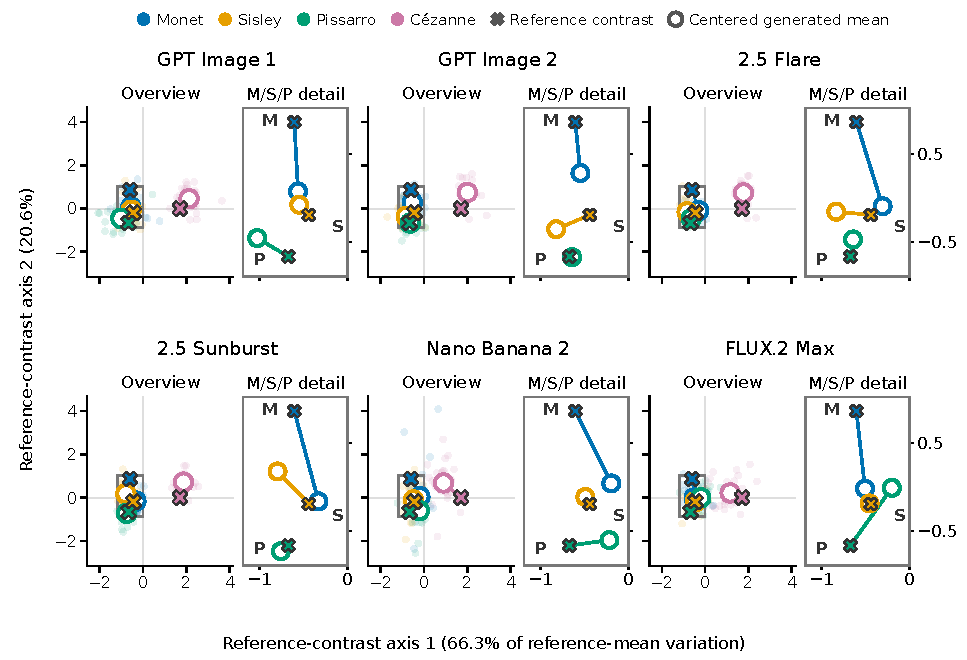
\includegraphics[width=\linewidth]{specificity_geometry.pdf}
\caption{Matching the labeled painter pattern. Crosses mark reference contrasts;
open circles average generated contrasts over all 14 scenes and both repeats.
Shorter matching-label lines indicate less projected mismatch;
faint dots show centered scene/repeat contrasts.
The outlined region is enlarged in the adjacent Monet (M), Sisley (S) and
Pissarro (P) detail at a common scale; C\'ezanne
remains in the overview. Each view uses common axes across models. Agreement
in these two projected axes does not establish agreement in all 31 features.}
\label{fig:specificity-geometry}
\end{figure}
\FloatBarrier

\subsection{Most scene-averaged change is common to the painter names}\label{sec:shared-change}
After averaging scenes, named-minus-artist-free shifts comprise a four-name mean
and painter-specific departures. The mean includes the oil-painting clause and
any common naming response: 82.5--95.7\% of repeat-corrected squared change
(Table~\ref{tab:shared-change}). Averaging emphasizes consistent shifts;
splitting within scenes retains scene-specific variation and gives 88.6--97.2\%
(Appendix~\ref{app:estimation}). $\beta$ measures departures along the reference contrasts.

\begin{table}[htbp]\centering\small\setlength{\tabcolsep}{3pt}
\begin{tabularx}{\linewidth}{@{}l*{6}{>{\centering\arraybackslash}X}@{}}
\toprule
& \shortstack{GPT Image\\1} & \shortstack{GPT Image\\2} & Flare & Sunburst & \shortstack{Nano\\Banana 2} & \shortstack{FLUX.2\\Max}\\\midrule
Shared (\%) & 82.5 & 85.8 & 84.8 & 83.9 & 88.1 & 95.7\\
Between-name (\%) & 17.5 & 14.2 & 15.2 & 16.1 & 11.9 & 4.3\\
\midrule
Corrected cosine & 0.689 & 0.774 & 0.766 & 0.837 & 0.930 & 0.916\\
Squared-size ratio & 1.986 & 1.960 & 2.816 & 3.356 & 3.692 & 4.138\\
\bottomrule\end{tabularx}
\caption{Shares of scene-averaged, repeat-corrected squared change from artist-free to named prompts, including the painting clause. Shared is the four-name mean shift; between-name is departure from it. The lower rows give retrospective comparisons of the shared named shift with the generic oil-painting shift, using the same artist-free baseline. The noise-corrected cosine measures their directional agreement (1 means parallel); the ratio divides their repeat-corrected squared magnitudes, shared by generic.}
\label{tab:shared-change}\end{table}


The shared named shift points broadly along the generic oil-painting shift
(noise-corrected cosine $.689$--$.930$; 1 means parallel), but its repeat-corrected
squared magnitude is 1.96--4.14 times as large. Both use scene averages and the
same artist-free baseline; Table~\ref{tab:shared-change} lists each model's values.
Thus, a response shared across painter names need not be identical to the response
to a generic painting instruction. The generic shift and the additional shared
naming shift can reinforce or oppose one another, so their squared magnitudes
do not add as independent contributions (Appendix~\ref{app:estimation}).
\FloatBarrier

\subsection{The aggregate response conceals uneven painter distinctions}
Retrospective pair diagnostics extend the lightness example in
Section~\ref{sec:contrast-intuition} to all 31 features (Figure~\ref{fig:artist-pairs}).
Monet--Sisley aligned responses range from $-.249$ to $.129$ in five models,
versus $.402$ for GPT Image 2. Yet GPT Image 1 has lower estimated error for this pair
($.56$ versus $1.16$): stronger alignment does not ensure lower mismatch.
Omitting C\'ezanne lowers FLUX's overall response from $.470$ to $.096$ and
GPT Image 2's from $.999$ to $.651$.

Swapping Monet and Sisley lowers error for Flare, Sunburst and Nano Banana 2.
Reversing a negatively aligned pair difference lowers error without changing its size.

\begin{figure}[!htbp]
\centering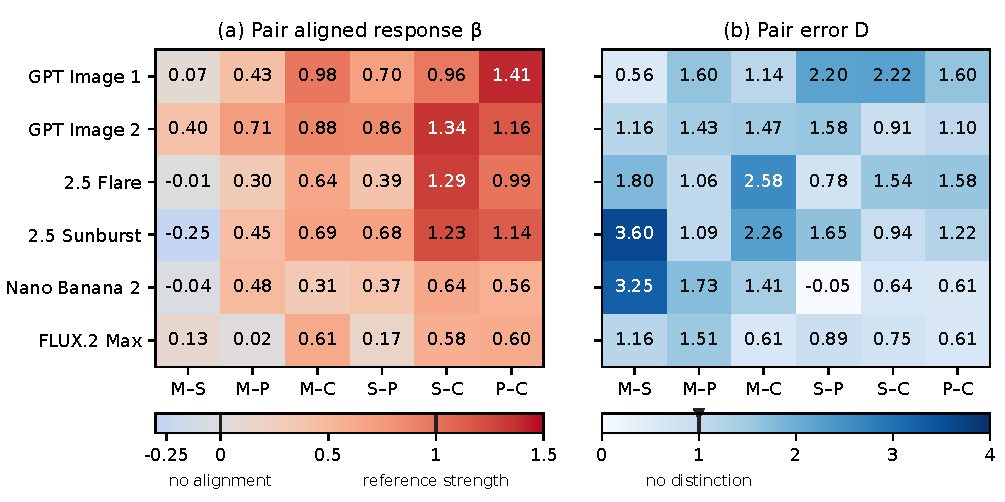
\includegraphics[width=\linewidth]{specificity_artist_pairs.pdf}
\caption{Descriptive painter-pair estimates (no pairwise tests). M, S, P and C denote Monet, Sisley,
Pissarro and C\'ezanne. Pair aligned response 0 means no aligned component,
1 matches reference strength, values above 1 exaggerate it, and negative values
indicate the opposite direction.
Expected error is 0 for exact agreement and 1 for no distinction. Each pair uses
all 31 features and is normalized by its squared reference distance.
Negative error can arise from repeat correction,
not better-than-exact agreement.}
\label{fig:artist-pairs}
\end{figure}
\FloatBarrier

\subsection{Scene averaging and contrast magnitude change the ordering}
We compare fit scene by scene, after averaging scenes, and after held-out
rescaling of painter contrasts (Table~\ref{tab:review-calibration}).

\emph{Averaging scenes.} Nano Banana 2's mean painter contrasts have lower error than FLUX's
($.723$ versus $.761$). Evaluating each scene adds a larger variation component
for Nano Banana 2 ($.387$ versus $.040$), reversing that order.
$D$ penalizes variation around the pooled historical target; averaging can
cancel scene-dependent differences.

\begin{table}[!htbp]\centering\small
\begin{tabularx}{\linewidth}{@{}l*{3}{>{\centering\arraybackslash}X}@{\hspace{2em}}>{\centering\arraybackslash}X@{}}\toprule
Model & \shortstack{Uncalibrated\\scene error\\$D$} & \shortstack{Error after\\averaging scenes\\$D_{\rm aggregate}$} & \shortstack{Scene\\variation\\$V_{\rm scene}$} & \shortstack{Calibrated\\scene error\\$D_{\rm held}$}\\
\cmidrule(r){1-4}\cmidrule(l){5-5}
GPT Image 1 & 1.572 & 1.239 & 0.333 & 0.645\\
GPT Image 2 & 1.226 & 1.044 & 0.182 & \textbf{0.554}\\
2.5 Flare & 1.738 & 1.483 & 0.255 & 0.741\\
2.5 Sunburst & 1.641 & 1.337 & 0.305 & 0.706\\
Nano Banana 2 & 1.109 & \textbf{0.723} & 0.387 & 0.832\\
FLUX.2 Max & \textbf{0.801} & 0.761 & 0.040 & 0.714\\
\bottomrule\end{tabularx}
\caption{Retrospective error decomposition and calibration against full-frame references. $D=D_{\rm aggregate}+V_{\rm scene}$. Calibration rescales centered generated contrasts using the other 13 scenes and evaluates them on the omitted scene; it does not produce new images. Bold marks each error column's minimum, not significance.}
\label{tab:review-calibration}\end{table}


\emph{Rescaling contrasts.} GPT Image 2's aligned response is near one, but its
squared contrast size exceeds twice the reference's ($Q=2.223$, where 1 matches the reference size;
Appendix~\ref{app:magnitude-coverage}).
Shrinking weakens its reference-aligned component, but reduces off-target
differences enough to lower the total error estimate. GPT Image 2's fitted multipliers
scale every contrast coordinate by about 0.45, using only the other 13 scenes each time.

After calibration, GPT Image 2 has the lowest error estimate, $.554$,
compared with FLUX's $.714$; it has lower scores in 12 of 14 held-out folds.
Deleting any scene and refitting the entire procedure preserves the mean
advantage (Appendix~\ref{app:magnitude-coverage}).
The folds overlap, so their win count does not establish statistical superiority.

\subsection{Which comparisons survive reference changes?}\label{sec:source-correction}
For the uncalibrated scene error $D$, FLUX retains the lowest point
estimate across scene deletions, measurement windows, reference targets and
feature-weighting sensitivities (Appendices~\ref{app:declared-sensitivities}
and~\ref{app:diagnostics}).

Source handling has a more consequential effect on statistical comparisons.
AI assistants inspected all reference and development reproductions, selecting
crops that exclude peripheral artifacts in 90 reference and 41 development images.
The audit used no human verification. After cropping and refitting development scaling,
FLUX's error estimate changes from $.801$ to $.872$. Corrected aligned-response
intervals remain above zero for all six models, and GPT Image 2 retains the lowest
calibrated estimate.

Table~\ref{tab:source-comparison} makes the changed comparisons explicit. With
corrected regions and refitted scaling, the Sunburst interval crosses zero,
Flare still has higher error than FLUX and the GPT Image 1 interval moves above zero. The latter
is a retrospective sensitivity, not a new confirmatory finding. Source correction
preserves FLUX's lowest point estimate while changing the evidence for particular
model differences.

\begin{table}[!htbp]\centering\small
\begin{tabularx}{\linewidth}{@{}Xcc@{}}\toprule
Model comparison & \shortstack{Full-frame difference\\{[adjusted interval]}} & \shortstack{Crop + scaling correction\\Difference [adjusted interval]}\\\midrule
GPT Image 1 $-$ FLUX & $0.771\;[-0.037,1.580]$ & $0.758\;[0.026,1.491]$\\[2pt]
2.5 Flare $-$ FLUX & $0.937\;[0.256,1.618]$ & $0.864\;[0.193,1.535]$\\[2pt]
2.5 Sunburst $-$ FLUX & $0.840\;[0.058,1.623]$ & $0.705\;[-0.026,1.436]$\\[2pt]
\bottomrule\end{tabularx}
\caption{Uncalibrated error differences before and after source correction, using audited painting regions and refitted development scaling. Positive differences favor FLUX.2 Max. Full-frame intervals use the 95\% simultaneous procedure across 21 endpoints; corrected intervals reuse that procedure retrospectively and add no confirmatory tests.}
\label{tab:source-comparison}\end{table}


\begin{samepage}
A separate check uses class-specific reference means for 11 water, built and
land briefs, excluding three mixed briefs. Replacing title-derived reference
labels with visual labels retains FLUX's lowest error estimate.
Appendix~\ref{app:diagnostics} gives the controls and audit.\par
\end{samepage}

\FloatBarrier

\section{Discussion}\label{sec:discussion}
The experiment separates reference-aligned name response, lower error on a
specified target, and faithful artistic reproduction. It supports the first
for all six configurations and two original comparisons under the second;
the Sunburst comparison loses adjusted separation after source correction. Neither
positive alignment nor a near-unit slope establishes low total error: GPT
Image 2's aligned amplitude coexists with substantial additional contrast.
FLUX's weaker response has lower uncalibrated error, while held-scene scalar
calibration favors GPT Image 2 in point estimates. Both evaluations are
coherent; neither defines a uniquely best artistic representation.

Aggregate alignment also conceals uneven coverage. The dominant reference
component receives stronger responses than the other components, and several
Monet--Sisley slopes are near zero or negative. These are weak measured pair
contrasts, not evidence of perceptual confusion or an identified art-historical
hierarchy. The generic clause shares part of the common named direction.
Shared non-additive transformations, content substitution and reproduction
processes remain possible explanations; training imbalance, preference
optimization and guidance were not manipulated. The separate palette and
fixed-map studies, including their contrary prospective result
(Appendix~\ref{sec:why}), do not establish a universal mechanism.

\subsection{Scope and remaining limitations}
The target is deliberately collection-relative. Scene-wise $D$ measures
consistency with pooled historical contrasts and can penalize appropriate
artist-by-content variation. Coarse content classes do not match composition,
viewpoint, career period or actual generated scene adherence. The source audit
addresses visible peripheral regions and title/visual-class disagreements; its
assistant judgments, unresolved boundaries and remaining capture differences
limit the correction. A single reproduction per work cannot identify effects
of illumination, sharpening, conservation or digitization source.

The coordinates measure digital properties, not physical brushwork or perceived
painter resemblance. The study makes no artistic-fidelity or internal-mechanism
claim. Weighting sensitivities and successful numerical replay establish neither.
Likewise, the real-painting control ranges mix finite-reference disagreement
with sparse sampling noise and do not define an artistic acceptance threshold.

Inference conditions on the reference panel and scaler. Simulations probe
specified noise models; they cannot verify actual repeat independence. Four
related painters, 14 authored briefs, two repeats and one clause template
restrict external inference. The image panels enable inspection, while the
remaining gap in public exact-pixel access limits independent measurement
reproduction.

\section{Conclusion}
Painter names produce reference-aligned digital contrasts beyond a common
additive response, but the alignment is uneven across painter distinctions.
Response strength, scene dependence and source handling change how configurations
compare. FLUX retains the lowest error estimate after region correction, but
its original adjusted Sunburst comparison does not persist; held-scene
calibration gives GPT Image 2 the lowest point estimate. These
findings distinguish detection, calibration and collection-relative agreement
without treating any one as a validated measure of artistic fidelity.

\section*{Data and code availability}
The \href{https://github.com/isingmodel/latent-art-bench}{repository} contains
protocols, prompts, request settings, source metadata, scalers and feature
vectors. The primary analysis, diagnostic extensions and source-quality
sensitivity have separate versioned records with input hashes and replay code.
The source audit records all work identities, region boxes, label decisions
and corrected vectors; the original results remain intact.

Appendix~\ref{app:images} displays 36 generated and four reference examples
with recorded identities and byte hashes. Public numerical replay begins with
vectors; independent re-extraction requires the exact source pixels, which
remain outside the compact repository. Earlier experiments have
\href{https://github.com/isingmodel/latent-art-bench/releases}{public releases};
the current experiment and corrections still need a dedicated public archive
with permissible exact pixels or a verified recovery route.

\bibliographystyle{plainnat}
\bibliography{references}

\appendix
\section{Feature definitions}\label{app:features}
Color coordinates use CIELAB under D65 and the $2^\circ$ observer. Lightness
and chroma each contribute a median and IQR. Chromatic fraction is the share
of pixels with $C^*\geq5$. Hue concentration is the magnitude of the
chroma-weighted circular mean; hue entropy uses 24 equally spaced bins and is
normalized by their log count. Both use chroma weights and are zero when fewer
than 1\% of pixels are chromatic. At each of three lags (1\%, 4\% and 16\% of
the short side), the median is taken over pooled horizontal and vertical
CIEDE2000 differences. A log--log slope summarizes their
scale dependence \citep{sharma2005ciede}.

Spatial and texture coordinates use linear-sRGB luminance. A Tukey window
(parameter .1) precedes Fourier analysis. Thirty-two logarithmic radial bins
cover 4--128 cycles per short side; a Theil--Sen line gives spectral slope and
its root-mean-square residual. Power-weighted axial concentration measures
anisotropy. Scharr derivatives supply gradient median and IQR, an 18-bin
magnitude-weighted orientation entropy, and horizontal--vertical balance. Mean
Jensen--Shannon divergence of quadrant orientation histograms from the global
histogram measures regional variation.

Four log mean-squared detail energies come from a four-level undecimated
\texttt{db2} wavelet transform, followed by their linear slope and mean second
difference \citep{mallat1989wavelet}. Uniform local-binary-pattern entropy uses
$(P,R)=(8,1),(16,2),(32,4)$ on quantized luminance
\citep{ojala2002lbp}. Three median local coefficients of variation use window
widths obtained by rounding 1\%, 4\% and 16\% of the short side and increasing
even widths to the next odd integer, with a $10^{-6}$ mean floor.
The fixed implementation records boundary handling and stabilizing
constants. The separate scaler contains 101 Monet, 36 Sisley, 48 Pissarro and
36 C\'ezanne works. Equal painter mass is used to calculate each weighted
median and IQR.

\section{Estimator details and sensitivity analyses}\label{app:estimation}
Let $\theta_{msa}=\mathbb E[d_{msak}]$ and
$d_{msak}=\theta_{msa}+\eta_{msak}$. If repeat errors have zero mean and
$\mathbb E\langle\eta_{msa1},\eta_{msa2}\rangle=0$, then
\[
 \mathbb E[\widehat D_{ms}]
 =H^{-1}\sum_a\|\theta_{msa}-r_a\|^2.
\]
Centering induces dependence between artists within a repeat, but independent
repeat blocks preserve the vanishing cross-repeat term. A common response has
$\theta_{msa}=0$ and hence expected $D=1$, even if it shifts the entire named
collection toward the references. A correctly aligned but rescaled response
$\theta_{msa}=b r_a$ gives expected $D=(b-1)^2$. Orthogonal deviations add their
squared magnitude. This identity explains why stronger painter contrasts need not have lower
reference-relative squared error.

For each model, global distortion applies the same cross-product estimator to
the scene-averaged contrasts. Its target differs from the mean scene-wise error through the variation term
in Equation~\ref{eq:scene-decomposition}; this term is not necessarily a failure. Both are reported,
without selecting the smaller as the primary result. The primary comparison
weights scenes and artists equally, irrespective of the reference count.
The report also retains each painter's additive contribution to $D$. These sum
to the model error but are not standalone artist-fidelity scores, because the
centering in Equation~\ref{eq:center} couples the four named conditions.

For a model contrast, compute one error difference per complete paired scene.
Its standard error is the sample standard deviation of those differences divided
by $\sqrt n$. The simultaneous half-width is
$t_{n-1,1-.05/(2\cdot21)}\,\mathrm{SE}$. Six slope intervals use the same
family adjustment. Additional nominal intervals and 5,000 paired-scene bootstrap
draws are descriptive checks, not alternative routes to significance. Reference
sensitivity draws 1,000 bootstrap samples independently within each painter,
recomputes reference means and $H$, and holds generated vectors and scaling
fixed. It describes reference-panel dependence rather than all uncertainty
jointly.

The four-class reference sensitivity uses a fixed lexicon applied to source
titles: water-organized, built-place-organized, route-organized, and open or
wooded land. Each class mean receives one-quarter weight within a painter.
Resampling within artist/class strata conditions on those labels and does not
account for classification error. The older controlled naming panel used a
separate three-class visual coding scheme, described below.

For the shared-effect diagnostic, average each arm over scenes within repeat.
With named-minus-free differences $h_{ak}$ and $c_k=\frac14\sum_a h_{ak}$,
common and specific squared magnitudes are $4\langle c_1,c_2\rangle$ and
$\sum_a\langle h_{a1}-c_1,h_{a2}-c_2\rangle$. Their common fraction is reported
when the total is positive; corrected components may be negative.
Let $g_k$ be the generic-minus-free shift. The ordinary repeat-averaged cosine
shares a noisy free estimate in both vectors, adding its error covariance trace
to the expected numerator. A separate diagnostic uses
$[\langle g_1,c_2\rangle+\langle g_2,c_1\rangle]/
[2\sqrt{\langle g_1,g_2\rangle\langle c_1,c_2\rangle}]$ when both norm squares
are positive. The ratio itself is not unbiased or constrained to $[-1,1]$.
Primary $D$ uses only named arms and is unaffected by shared-free-control noise.

\section{Post-result target diagnostics}\label{app:diagnostics}
These retrospective analyses retain the completed 1,008 generated images and
the original inferential family. The initial diagnostics use unchanged reference
vectors and scaling; the subsequent source audit separately varies painting
regions, development scaling and content labels.

\subsection{Content-specific targets and genuine-painting controls}
The recorded reference classes are water-organized, built-place-organized,
route-organized, and open or wooded land, assigned by a fixed source-title
lexicon. Counts in that order are $(191,67,8,31)$ for Monet, $(52,29,9,16)$ for
Sisley, $(28,77,12,24)$ for Pissarro and $(31,28,12,34)$ for C\'ezanne.
Class-specific means are centered across painters just as in the pooled target.
Their mean squared departure from the pooled target is $.438H$, a description
of observed reference means that includes finite-sample error.

For the generated comparison, the four water, four built and three land briefs
use the corresponding class means; the three mixed briefs are excluded.
We average the class-specific cross-product error over these $S=11$ scenes and divide by
$H_c=S^{-1}\sum_s\sum_a\|r_{a,c(s)}\|^2=7.413$, compared with pooled $H=5.915$.
Each column of Table~\ref{tab:review-targets} therefore has its own denominator.
The unchanged 11-scene pooled comparison isolates the scene-subset choice.
These title-derived strata have 16--191 reference works per artist/class among
the three included classes, but do not supply visually matched historical scenes.

For each of 1,000 genuine-painting controls, works in each artist/class cell
are randomly divided into disjoint halves, with the smaller half used for
target estimation. A pooled control samples two independent works with replacement
from each painter's held-out half for each of 14 pseudo-scenes. A class-stratified
control samples within the held-out class for each of the 11 water, built or
land pseudo-scenes. It is compared with both pooled and class-specific means
from the training halves, using each target's own squared magnitude.
The random seed is 2026091201. Sampling can repeat a held-out work, but no
held-out work is used to estimate that split's target. The development scaler
is fixed throughout.

To separate sparse sampling from changes in the comparison pools, we also
calculate each split's expected score from its exact held-out means, keeping
the training target and normalizer fixed (Table~\ref{tab:painting-control-ranges}).

\begin{table}[htbp]
\centering\small
\begin{tabular}{llcc}
\toprule
Control sampling & Reference target & Two draws & Exact held-out means\\
\midrule
Pooled & Pooled & $[-.758,1.380]$ & $[.135,.428]$\\
Class-stratified & Pooled & $[-.554,2.400]$ & $[.544,.993]$\\
Class-stratified & Class-specific & $[-.248,1.946]$ & $[.517,.954]$\\
\bottomrule
\end{tabular}
\caption{Central 95\% ranges of genuine-painting control scores across 1,000
splits. Exact means integrate out sampling within each split; these finite-pool
ranges are not confidence intervals.}
\label{tab:painting-control-ranges}
\end{table}

For pooled controls, SD falls from $.561$ to $.076$ after integrating out
sampling. These controls still condition on imperfect title classes and a
single source capture per work; they do not calibrate artistic fidelity.

\begin{table}[htbp]\centering\small
\begin{tabular}{@{}lrrrr@{}}\toprule
 & \multicolumn{2}{c}{11 common briefs} & \multicolumn{2}{c}{14 briefs}\\
Model & Pooled target & Class target & Equal family & Covariance\\\midrule
GPT Image 1 & 1.557 & 1.366 & 1.551 & 2.103\\
GPT Image 2 & 1.099 & 1.130 & 1.243 & 1.511\\
2.5 Flare & 1.726 & 1.539 & 1.765 & 1.636\\
2.5 Sunburst & 1.633 & 1.525 & 1.680 & 1.617\\
Nano Banana 2 & 0.987 & 0.948 & 1.203 & 1.385\\
FLUX.2 Max & 0.750 & 0.786 & 0.808 & 0.928\\
\bottomrule\end{tabular}
\caption{Descriptive error under alternative targets and metrics. The class target uses title-derived water, built and land strata; the three mixed briefs are excluded. Each column uses its own reference normalizer; absolute values across columns are not directly comparable. Covariance is fitted only on development works, with fixed 50\% shrinkage.}
\label{tab:review-targets}\end{table}

\FloatBarrier

\subsection{Magnitude, artist coverage and coordinate weighting}\label{app:magnitude-coverage}
The cross-repeat version of Equation~\ref{eq:scene-decomposition} is exact for
the retained vectors. Its variation term replaces squared deviations with
cross-products between scene-centered repeats. The term can be negative in
finite samples, although its independent-repeat population target is nonnegative.
Scalar calibration fits only the other 13 scenes. All fold denominators $Q$
are positive. GPT Image 2's fitted scalars range from .438 to .459 and FLUX's
from .598 to .694; all fold-specific scores are retained. No calibration
parameter is selected by minimizing its own held-out score. The subsequent
deletion check refits the entire procedure on
each remaining 13-scene panel, rather than treating overlapping folds as
independent replications. Its mean GPT Image 2-minus-FLUX error differences
range from $-.189$ to $-.137$.

\begin{table}[htbp]\centering\small
\begin{tabular}{@{}lrr@{}}\toprule
Model & Squared contrast magnitude $Q$ & Alignment ratio $\beta/\sqrt Q$\\
\midrule
GPT Image 1 & 2.449 & 0.600\\
GPT Image 2 & 2.223 & 0.670\\
2.5 Flare & 2.281 & 0.511\\
2.5 Sunburst & 2.289 & 0.545\\
Nano Banana 2 & 0.994 & 0.444\\
FLUX.2 Max & 0.741 & 0.546\\
\bottomrule\end{tabular}
\caption{Descriptive magnitude and alignment of painter contrasts. $Q=1$ equals the reference squared size, and $D=1-2\beta+Q$. The alignment ratio can fall outside $[-1,1]$ in finite samples.}
\label{tab:review-alignment}\end{table}


For artist pairs, both generated and reference contrasts are direct differences
between the two artists; the denominator is the squared reference-pair distance.
Leaving one artist out recenters the remaining three generated and reference
conditions. Reference singular components are the three rank-one terms of the
centered four-by-31 reference matrix: each combines an artist contrast with a
feature direction, rather than representing one artist. Component aligned
responses project onto each term separately.

\begin{table}[htbp]\centering\small
\begin{tabular}{@{}lrrr|rrrr@{}}\toprule
 & \multicolumn{3}{c}{Component aligned response} & \multicolumn{4}{c}{Aligned response after omitting}\\
Model & First & Second & Third & Monet & Sisley & Pissarro & C\'ezanne\\\midrule
GPT Image 1 & 1.248 & 0.310 & 0.356 & 1.140 & 1.072 & 0.840 & 0.389\\
GPT Image 2 & 1.156 & 0.617 & 0.800 & 1.195 & 0.972 & 0.992 & 0.651\\
2.5 Flare & 1.022 & 0.211 & 0.383 & 1.034 & 0.734 & 0.802 & 0.222\\
2.5 Sunburst & 1.082 & 0.250 & 0.417 & 1.116 & 0.840 & 0.762 & 0.284\\
Nano Banana 2 & 0.513 & 0.371 & 0.195 & 0.569 & 0.446 & 0.388 & 0.276\\
FLUX.2 Max & 0.666 & 0.021 & 0.183 & 0.539 & 0.511 & 0.527 & 0.096\\
\bottomrule\end{tabular}
\caption{Descriptive artist coverage of the aligned response. Reference components account for 66.3\%, 20.6\% and 13.0\% of centroid variation. Each omission recomputes the target and recenters the other three artists.}
\label{tab:review-components}\end{table}


Table~\ref{tab:review-components} shows that aggregate positive alignment is
uneven across those components.

Equal-family weighting assigns each coordinate inverse family size (11, 8 or 12).
The covariance sensitivity uses 221 development works with equal painter mass.
For their weighted covariance $\Sigma$, the metric is
$[.5\Sigma+.5\operatorname{tr}(\Sigma)I/31]^{-1}$, with fixed shrinkage and no
tuning on evaluated images. These weighting choices are not independently
validated artistic metrics.

\begin{samepage}
FLUX retains the lowest point estimate under all
31 single-coordinate deletions; the report retains every coordinate contribution,
including negative terms.
Without texture, Flare and Sunburst still have error estimates above the
no-contrast value of one (1.580 and 1.604).
\end{samepage}

\subsection{A design-aware energy correction}
The primary energy values use empirical distributions, including their zero
diagonal distances. To estimate energy between a fixed empirical reference
and the equally weighted mixture of scene-conditional output distributions,
cross-scene generated pairs already have the required independent draws.
Only the same-scene generated term needs adjustment. With two repeats and
$S$ scenes, the descriptive correction is
\[
 \widehat{\mathcal E}_{\rm strata}
 =\widehat{\mathcal E}_{\rm empirical}
 -\frac{1}{2S^2}\sum_s\|y_{s1}-y_{s2}\|.
\]
The reference within-distance remains empirical because this target conditions
on the finite reference panel. A pooled IID $n/(n-1)$ multiplier would also
alter cross-scene terms and estimate a different target. This correction retains
the 21 negative named-minus-generic differences. It does not solve unequal
historical and generated content mixtures, and no new energy tests are performed.

\subsection{Uncertainty and synthetic coverage checks}
The Student procedure uses 14 scene summaries. For independent scene errors
with fixed conditional means $\delta_s$, its estimated variance has expectation
\[
 \mathbb E[s_\delta^2/S]
 =\operatorname{Var}(\bar{\widehat\delta})
 +\frac{1}{S(S-1)}\sum_s(\delta_s-\bar\delta)^2.
\]
It therefore includes real between-scene heterogeneity as well as request noise.
This explains why it is not a direct estimate of fresh-request variance for
exactly the fixed panel. It also does not provide an exact coverage guarantee:
non-Gaussian cross-products and dependence can affect the Student approximation.

The initial 5,000-run scenarios (seed 2026091202) use the six configurations,
14 scenes, two repeats and 21-endpoint family, with unit reference magnitude.
Gaussian, variance-standardized $t_3$/heteroskedastic and fixed scene-interaction
errors give simultaneous coverage 95.96\%, 97.42\% and 99.68\%. Their independent
centered noise power is $.5$. Allocating half the noise to a model-specific
state shared by all scenes and both repeats reduces coverage to 0.04\%, with
mean corrected-error bias near $.25$.

A subsequent sweep uses independent Gaussian errors at powers $.5$, $1.5$ and
$3$, with either isotropic or rank-three covariance aligned with the reference
components (5,000 runs per case). Coverage ranges from 95.06\% to 96.80\%, with
Monte Carlo SE $.25$--$.31$ percentage points. For comparison, directly centered
repeat differences estimate observed powers of $.424$--$2.596$ relative to $H$.
These stress models probe coverage approximations, not actual service independence;
no significance threshold is selected from them.

\subsection{Source-quality sensitivity}\label{app:reference-quality}
AI assistants inspect all 649 reference and 221 development reproductions
using contact sheets and enlarged peripheral regions, recording removable
calibration targets, frames, margins and labels. Uncertain boundaries remain
unchanged. Reference content is visually classified before comparison with the
title label; mixed or unclear cases retain that label.

The audit selects crops for 90 reference and 41 development images, including
ten calibration-strip cases; 43 uncertain boundaries remain unchanged. Visual
classes differ from 230 title assignments, while 42 mixed or unclear cases
retain their original labels. These AI-coded sensitivities did not undergo human verification and are not
independent ground truth.

Audited rectangular crops follow the original orientation and ICC rules, before
aspect-preserving Lanczos resizing to a 512-pixel short side without upsampling.
All 31 features and all works are retained. We compare corrected references with
original scaling, then refit development IQR scaling and consistently transform
generated vectors. Label sensitivity uses the same 11 briefs. Versioned records
preserve audit decisions, new vectors and original results; model scores do not
select corrections.
All six aligned-response intervals remain above zero with either scaler.
With original scaling, corrected regions give FLUX $D=0.832$.
After refitting, (uncalibrated, held-out calibrated) errors are:
GPT Image 1 $(1.631,0.693)$, GPT Image 2 $(1.259,0.579)$,
Flare $(1.737,0.760)$, Sunburst $(1.577,0.711)$, Nano Banana 2 $(1.121,0.846)$
and FLUX $(0.872,0.762)$. FLUX and GPT Image 2 retain the respective minima.

\section{Image selection and provenance}\label{app:images}
The generated examples use the first declared brief and first repeat, selected
after analysis without appearance- or score-based curation. The brief reads:
``A broad river bends past a gravel bank. Three tall trees stand on the far bank,
with a low hill behind them under a pale overcast sky.'' Every prompt ends with
``No text or frame.'' Only the clauses in Section~\ref{sec:design} change.

References in Figure~\ref{fig:original-generated} are the lexicographically first
measured work IDs per painter classified as water-organized in the completed
audit, with recorded public-domain status. The Sisley and Pissarro reproductions
use audited crops removing calibration strips; Monet and C\'ezanne retain their
full regions. The manifest records image identities, provenance, crop boxes
and exact prompts. The paintings are not matched to the generated brief.


\FloatBarrier


\section{Complete model and painter summaries}\label{app:results}
Table~\ref{tab:all-specificity-pairs} reports the full model-comparison family;
Table~\ref{tab:artist-distributions} retains distributional outcomes for every
painter and model. The latter do not inherit the primary model-contrast
significance tests. Their energy values concern empirical distributions of
28 named or generic outputs against the recorded reference panel.
\begin{table}[htbp]\centering\small
\begin{tabular}{llr}\toprule
Model A & Model B & $D_A-D_B$ [simultaneous interval]\\\midrule
GPT Image 1 & GPT Image 2 & $0.346\;[-0.400,1.093]$\\
GPT Image 1 & 2.5 Flare & $-0.165\;[-1.027,0.697]$\\
GPT Image 1 & 2.5 Sunburst & $-0.069\;[-1.181,1.043]$\\
GPT Image 1 & Nano Banana 2 & $0.463\;[-0.602,1.528]$\\
GPT Image 1 & FLUX.2 Max & $0.771\;[-0.037,1.580]$\\
GPT Image 2 & 2.5 Flare & $-0.512\;[-1.150,0.126]$\\
GPT Image 2 & 2.5 Sunburst & $-0.415\;[-1.181,0.350]$\\
GPT Image 2 & Nano Banana 2 & $0.116\;[-0.922,1.155]$\\
GPT Image 2 & FLUX.2 Max & $0.425\;[-0.161,1.011]$\\
2.5 Flare & 2.5 Sunburst & $0.096\;[-0.286,0.478]$\\
2.5 Flare & Nano Banana 2 & $0.628\;[-0.283,1.540]$\\
2.5 Flare & FLUX.2 Max & $0.937\;[0.256,1.618]$\\
2.5 Sunburst & Nano Banana 2 & $0.532\;[-0.436,1.500]$\\
2.5 Sunburst & FLUX.2 Max & $0.840\;[0.058,1.623]$\\
Nano Banana 2 & FLUX.2 Max & $0.309\;[-0.847,1.464]$\\
\bottomrule\end{tabular}
\caption{All 15 paired model comparisons in the prespecified inferential family. Intervals are approximate 95\% simultaneous intervals adjusted across all 21 endpoints. A negative contrast favors model A on the stated feature-geometry target.}
\label{tab:all-specificity-pairs}\end{table}

\begin{table}[htbp]\centering\small
\begin{tabular}{llrrrr}\toprule
Model & Measure & Monet & Sisley & Pissarro & C\'ezanne\\\midrule
GPT Image 1 & Energy change & $-2.515$ & $-2.739$ & $-2.628$ & $-1.336$\\
& Variance ratio & $0.479$ & $0.694$ & $0.603$ & $0.598$\\
\addlinespace[2pt]
GPT Image 2 & Energy change & $-0.602$ & $-1.092$ & $-0.195$ & $-0.373$\\
& Variance ratio & $0.283$ & $0.312$ & $0.303$ & $0.303$\\
\addlinespace[2pt]
2.5 Flare & Energy change & $0.962$ & $-0.008$ & $0.429$ & $-1.013$\\
& Variance ratio & $0.269$ & $0.371$ & $0.321$ & $0.275$\\
\addlinespace[2pt]
2.5 Sunburst & Energy change & $0.267$ & $-0.718$ & $-0.091$ & $-1.653$\\
& Variance ratio & $0.248$ & $0.274$ & $0.273$ & $0.318$\\
\addlinespace[2pt]
Nano Banana 2 & Energy change & $-0.513$ & $-1.381$ & $-0.741$ & $-1.102$\\
& Variance ratio & $0.829$ & $0.708$ & $0.572$ & $0.877$\\
\addlinespace[2pt]
FLUX.2 Max & Energy change & $-0.707$ & $-0.886$ & $-1.080$ & $-1.431$\\
& Variance ratio & $0.340$ & $0.416$ & $0.570$ & $0.622$\\
\bottomrule\end{tabular}
\caption{Complementary empirical distribution summaries. Energy change is named-minus-generic reference energy; variance ratios are generated-to-reference. Negative changes favor naming; ratios below one indicate narrower generated feature distributions.}
\label{tab:artist-distributions}\end{table}

\FloatBarrier

\begin{figure}[tbp]
\centering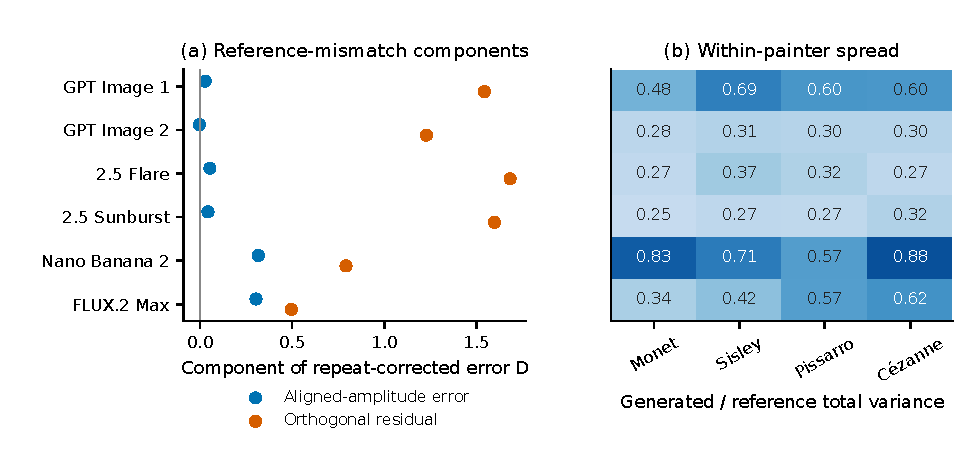
\includegraphics[width=\linewidth]{specificity_diagnostics.pdf}
\caption{Complementary descriptive summaries. (a) Reference-aligned amplitude
error and the residual orthogonal to the stacked reference configuration.
(b) Generated/reference variance ratios for every model and painter. Total
spread includes variation across fixed briefs and is not a mode-collapse measure.}
\label{fig:specificity-diagnostics}
\end{figure}
\begin{figure}[tbp]
\centering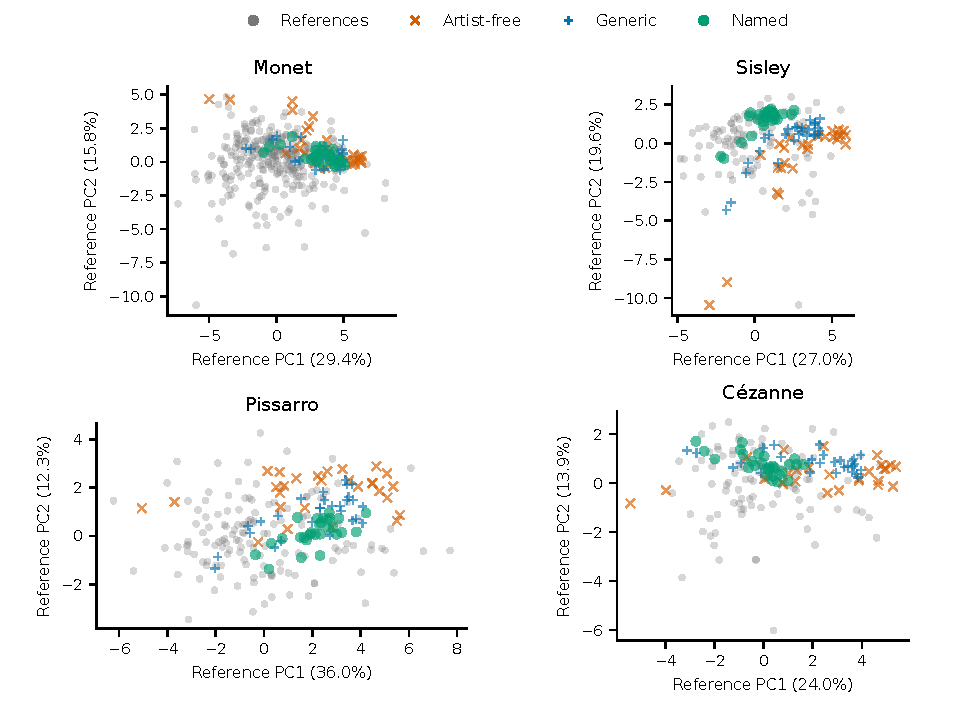
\includegraphics[width=.92\linewidth]{specificity_sunburst_distributions.pdf}
\caption{All four painters' reference and generated distributions, illustrated
with GPT Image 2.5 Sunburst. This model illustration was selected before the
primary feature outcomes were inspected. Each panel uses principal components
fitted only to that painter's reference works, so axes differ between painters.
The 14 generated briefs and two repeats have a different content distribution
from the historical panel. Projections are descriptive; numerical summaries
use all 31 coordinates.}
\label{fig:specificity-distributions}
\end{figure}
\FloatBarrier

\section{Supporting interventions}\label{sec:why}\label{app:cohorts}
These earlier cohorts address related but different questions
(Table~\ref{tab:cohorts}). They are not pooled with the six-model experiment
or treated as independent-investigator replications.

\begin{table}[htbp]
\centering\small
\begin{tabularx}{\linewidth}{@{}>{\raggedright\arraybackslash}p{.22\linewidth}>{\raggedright\arraybackslash}p{.27\linewidth}>{\raggedright\arraybackslash}X@{}}
\toprule
Cohort & Comparison & Role in this paper\\
\midrule
Four-painter exploration & 649 references; 1,920 generated outputs &
Describes reference/generated separation and motivates the controlled test.\\[4pt]
Controlled naming & 1,006 outputs; 38 Monet and 32 C\'ezanne references &
Six named/free and two detailed/short prompt contrasts; subsequent transformation
and conditional-variance diagnostics.\\[4pt]
Palette interventions & Two separate 192-output collections &
Named-minus-generic chroma response; no pooling across collections.\\[4pt]
Generic-clause comparison & 96 C\'ezanne/generic outputs on 24 new scenes &
Tests a proximity gain beyond a generic painting clause.\\[4pt]
Fixed-map transfer & 240 FLUX/C\'ezanne outputs on 12 new scenes &
Prospective counterexample to the historical opposing energy/prediction ordering.\\
\bottomrule
\end{tabularx}
\caption{Supporting evidence is kept separate from the new six-model experiment.
Different prompts, panels and finite-sample targets do not form one pooled test.}
\label{tab:cohorts}
\end{table}

\subsection{Proximity and spread under naming}
The four-painter exploration used 1,536 named and 384 artist-free outputs,
three prompt methods and 16 scenes. Its 24 model--painter--method cells had
trace ratios .206--.376 and grouped generated/reference discrimination accuracy
.940--.983. Pooled named energy medians for Monet, Sisley, Pissarro and C\'ezanne
were 2.068, 1.678, 1.975 and 2.142; corresponding artist-free medians were
1.732, 1.878, 1.854 and 1.657. Only Sisley had a lower pooled named median.
Matched-size real/real medians were .193, .215, .164 and .199. These post-result
summaries describe that exploration, not a general naming effect.

The later controlled panel selected Monet and C\'ezanne after exploration.
It crossed 24 scenes with three models, two clauses and three repeats; 142
short-scene outputs supplied two prompt-length comparisons. Reference panels
contained 38 Monet and 32 C\'ezanne works, with water/built/land masses based on
maintainer-run LLM visual coding. Named-minus-free energy changes were
$-.846,-1.818$ for Nano Banana 2, $-.625,-.896$ for FLUX, and $-.234,-.056$ for
GPT Image 2 (Monet, C\'ezanne). The first four rejected in the original family
of eight. A separate 72-output FLUX collection repeated both directions
($-.695,-.952$) with rejection in its own four-endpoint family.

A standalone 96-output C\'ezanne comparison on 24 new scenes reduced energy
relative to the generic clause by 1.195 ($p=.00001$, fixed $\alpha=.025$), with
named/generic trace ratio .552. It randomized clauses within 48 two-position
blocks, used reference class masses $(3,11,18)/32$, and tested a sharp no-effect
null with 99,999 within-block sign draws and plus-one correction. This tests
clause effects, not equality of energy alone. A generic clause therefore did
not reproduce the full proximity gain in that panel, but proximity does not
establish correct four-artist contrasts. Likewise, lower total spread does
not establish loss of scene information: controlled FLUX/Monet held-repetition
scene retrieval rose from 44.4\% to 59.7\% under naming. This measures relative
feature distinguishability, not verified prompt adherence.

\subsection{Palette responsiveness and a contrary transfer result}
Two separate 192-output palette collections used six scenes, four repeats,
muted/vivid instructions and free, generic, Monet and C\'ezanne clauses. The
primary name-minus-generic chroma-response interactions were unresolved:
$-.284,-.018$ in the first collection and $-.159,.037$ in the later one.
Their respective adjusted intervals spanned zero; the original family had
two interactions and the later family included two additional FLUX endpoints.
Secondary generic-minus-free responses were $-.853$ and $-.891$, with nominal
95\% intervals excluding zero. Thus generic painting can attenuate measured
palette response without an identified additional name effect. Two palette
levels do not distinguish reduced gain from saturation or an operating-range
shift, and unresolved interactions do not demonstrate equivalence.

Historical generated-only moment maps were fitted on training scenes and
assessed on held-out scenes. Actual naming had lower reference energy than
translation plus isotropic scaling in all six model--painter averages. Adding
scale improved named-mean prediction in all six while worsening reference
energy in five. That ordering did not transfer to a prospective 240-output
FLUX/C\'ezanne comparison with 12 new scenes and ten repeats, using the original
fits unchanged. Translation/scaling improved both energy and repeat-corrected
prediction error relative to translation: $-.390\;[-.509,-.271]$ and
$-5.047\;[-7.880,-2.214]$, with approximate simultaneous jackknife intervals.
The achieved prediction-error half-width exceeded its planning criterion.
This contrary result is retained without extra sampling; it rules out treating
the historical opposing ordering as a universal mechanism. These fitted
named/free maps are distinct from the review-driven artist-contrast scalar
counterfactual in Table~\ref{tab:review-calibration}.

\section{Collection provenance and computational scope}\label{app:provenance}
Historical GPT Image 1 and GPT Image 2 labels identify the requested model
names. A later technical negative control showed that the earlier image
interface also accepted an invented image-model identifier. This does not show
that valid names select the same underlying model, but successful request
acceptance alone cannot authenticate their separation. Historical contrasts
are therefore interpreted as recorded request-group comparisons. The current
experiment uses explicit documented model identifiers and fixed routes;
it does not reuse historical images as verified examples of the new variants.
All current outputs decode to the requested square dimensions, but their
response bodies do not echo model or quality fields. Labels therefore denote
the documented request configurations, without independent checkpoint
attestation. Underlying checkpoints and training corpora are not available
for inspection.

The present experiment excludes technical probes and an earlier attempt closed
before feature measurement because model selection could not be qualified.
No image is shared between these collections. The earlier incomplete
generic-clause cohort is likewise not pooled with its complete 96-image
successor. Exact assignments, attempt outcomes and measurement exclusions are
retained in the versioned manifests; selection was not based on visual success.
\end{document}
